\begin{thm}{226}{\hosi 2}{慶大 総合政策 (2017)}
 半円Hが6つの円A, $\ldots$, Fを含む。B, C, Dは全て合同で、BとC、CとDは接している。E, Fは合同で、EはBとCに、FはCとDに接している。E, Fは半円Hの円弧と直径に接している。Aの下に接する直線はE, Fと接している。Aの半径が1のとき、B, Hの半径を求めよ。
 \begin{center}
  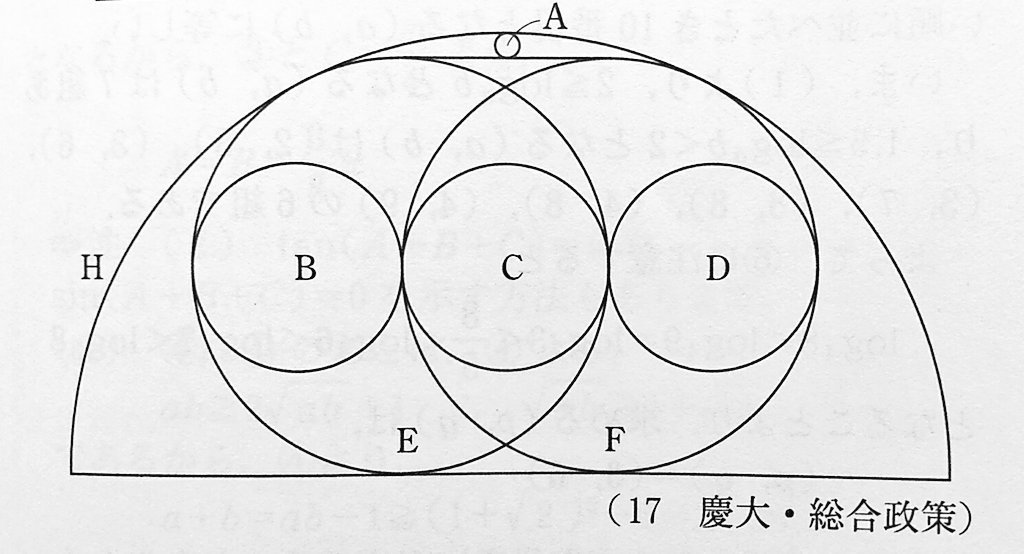
\includegraphics[bb=0 0 1024 554,width=0.7\linewidth]{../problems/Q_226/Q_226.jpg}
 \end{center}
\end{thm}

B,C,Dの半径を$x$、E,Fの半径を$y$とする。\\
Eの直径$=$Bの直径+Cの直径より $y=2x$\\
Hの半径はEの直径+Aの直径なので$2y+2=4x+2$\\
Hの中心をOとし, B,Cの交点をKとすると\\
OKの長さは三平方の定理から $\sqrt{x^2+(2x)^2}~\sqrt{5}x$\\
EとHの円弧との接点をLとすると, KLはEの半径$2x$に等しい。\\
よって, OL$=(2+\sqrt{5})x$\\
これはHの半径にも等しいので OL$=4x+2$\\
この2式から, Bの半径は$x=\dfrac{2}{\sqrt{5}-2}=4+2\sqrt{5}$\\
Hの半径は $(2+\sqrt{5})x=18+8\sqrt{5}$ 
